% Working draft of the paper planned from this project.
% Build: cd paper && tectonic main.tex
% \todo{...} marks what still has to be done or decided; it prints in bold brackets.
\documentclass[aps,prb,reprint,superscriptaddress,nofootinbib,floatfix]{revtex4-2}

\usepackage{amsmath,amssymb,bm}
\usepackage{graphicx}
\usepackage{booktabs}
\usepackage[hidelinks]{hyperref}   % black-and-white: no coloured links

\newcommand{\todo}[1]{\textbf{[TODO: #1]}}
\newcommand{\figplaceholder}[2]{%
  \fbox{\parbox[c][#1][c]{0.94\linewidth}{\centering\small\textit{Planned figure:} #2}}}
\newcommand{\cm}{\ensuremath{\text{cm}^{-1}}}
\newcommand{\chizero}{\bm{\chi}_0}
\newcommand{\muzero}{\bm{\mu}_0}
\newcommand{\lam}{\bm{\lambda}}

\begin{document}

\title{Does vibrational strong coupling reorganize the hydrogen-bond network of liquid
water? Polarizable machine-learning cavity molecular dynamics}
% \todo: final title once the liquid-water results are in.

\author{Charlie Wade}
\affiliation{Department of Physics, City College of New York, New York, New York 10031, USA}
\author{\todo{co-authors, e.g.\ model training / experimental collaborators}}
\noaffiliation
\author{Johannes Flick}
\email{jflick@ccny.cuny.edu}
\affiliation{Department of Physics, City College of New York, New York, New York 10031, USA}
\affiliation{Department of Physics, The Graduate Center, City University of New York, New York, New York 10016, USA}
\affiliation{Center for Computational Quantum Physics, Flatiron Institute, New York, New York 10010, USA}

\date{\today}

\begin{abstract}
Infrared experiments on liquid water in Fabry--P\'erot cavities indicate that
vibrational ultra-strong coupling of the O--H stretch slows the thermal disordering of
the hydrogen-bond network and redistributes water between network, intermediate and
isolated configurations, without any external driving. A microscopic explanation is
missing: in classical cavity molecular dynamics with fixed-charge models, the cavity
cannot change equilibrium structure at all, so such simulations are blind to this
effect by construction. Here we use \texttt{cboamd}, a cavity Born--Oppenheimer
molecular-dynamics framework that includes the electronic polarizability, the minimal
ingredient through which a cavity can bias thermal equilibrium. We first validate the
approach on a single CO$_2$ molecule, reproducing published polariton branches, and on
a single water molecule, whose bend polaritons split linearly with coupling. We then
follow the collective coupling from one to a few water molecules, establishing
\todo{$\sqrt{N}$ scaling / separation and orientation dependence}. Finally, with
machine-learned models for the energy, dipole moment and polarizability of liquid
water, we simulate the O--H stretch polaritons of the liquid and find that
\todo{main result: whether and how the hydrogen-bond populations, their temperature
dependence and the polariton linewidths change, and by how much compared with
experiment}. \todo{One closing sentence on what this means for cavity-modified
chemistry in water.}
\end{abstract}

\maketitle

% ---------------------------------------------------------------------------
\section{Introduction}

When molecular vibrations interact strongly with the confined electromagnetic field of
an optical cavity, they hybridize with the cavity mode into vibrational polaritons. In
this regime of vibrational strong coupling (VSC), the infrared (IR) absorption peak of
the molecules splits into a lower and an upper polariton separated by the Rabi
splitting, which grows with the square root of the number of coupled
molecules~\cite{Shalabney2015,Thomas2016}. What makes VSC remarkable is that it appears
to change matter itself: placing reacting solutions in a resonant infrared cavity, in
the dark, has been reported to slow reactions, change their selectivity and modify
energy transfer~\cite{Thomas2016,Thomas2019,Xiang2020,Ahn2023}. At the same time,
careful attempts to reproduce some of these effects found much smaller changes or none
at all~\cite{Imperatore2021,Wiesehan2021}. Why, and when, a cavity alters the ground
state of a molecular ensemble remains an open question.

Water is the natural place to ask this question. It is the solvent of most of
chemistry and biology, and its properties are set by a flexible hydrogen-bond network.
Its O--H stretch is one of the strongest infrared absorbers, so liquid water reaches
the strong- and even ultra-strong-coupling regimes readily. Experiments have reported
that collective VSC of water raises its ionic conductivity~\cite{Fukushima2022}. Most
recently, Itatani \textit{et al.}\ resolved the O--H stretching band of water under
vibrational ultra-strong coupling into contributions from network, intermediate and
isolated molecules~\cite{Itatani2026}. They found that the thermal disordering of the
hydrogen-bond network is retarded inside the cavity, that the fractions of
intermediate and isolated water grow anomalously at elevated temperature, and that the
upper polariton narrows towards the homogeneous linewidth of single water molecules.
They interpret these observations as vacuum-field-mediated correlations between water
molecules that extend beyond those of bulk water. A spectrum alone, however, cannot say
which hydrogen bonds change, or why.

Molecular dynamics (MD) simulations can, because they follow every molecule. Cavity MD
with empirical force fields has been applied to liquid water under VSC and reproduces
the polariton splitting of the O--H stretch~\cite{Li2020PNAS,Lieberherr2023}, as does
an extended cavity Born--Oppenheimer treatment~\cite{Bowles2025}. Where the structure
of the liquid was examined, it changed little~\cite{Li2020PNAS,Bowles2025}. This is not an accident. For a
fixed-charge model, the photon coordinate is a harmonic oscillator whose center depends
on the nuclear positions but whose curvature does not; integrating it out of the
classical partition function gives a constant, so every equilibrium average of the
nuclei is identical inside and outside the cavity~\cite{Li2020JCP}. A classical
simulation can only see a cavity-induced change of the hydrogen-bond network if the
coupling depends on the configuration in a way that goes beyond a fixed dipole. In
addition, fixed-charge models misrepresent the light--matter coupling itself: an
inaccurate dipole surface directly distorts the Rabi splitting, and for water the
widely used q-TIP4P/F model underestimates the O--H stretch intensity and therefore its
splitting~\cite{Lieberherr2023}.

The cavity Born--Oppenheimer approximation (CBOA)~\cite{Flick2017} provides a
first-principles route that avoids both problems. In its effective electric-field
formulation~\cite{Bonini2024}, the coupled nuclear--photon dynamics depend only on
three field-free properties of the matter: the ground-state energy, the dipole moment
and the polarizability. All three can be computed with standard electronic-structure
codes and learned by machine-learning interatomic potentials (MLIPs). The resulting
framework, \texttt{cboamd}~\cite{Li2026cboamd}, makes collective VSC in the condensed
phase accessible at near first-principles accuracy. Crucially, the polarizability
screens the cavity field in a configuration-dependent way. This renormalizes the
effective cavity frequency, the molecular analogue of the refractive index of the
intracavity medium, and it is the minimal classical mechanism through which the cavity
vacuum can bias thermal equilibrium~\cite{Li2026cboamd}. For liquid CO$_2$ the same
framework predicts strongly modified IR spectra but an unchanged pair
structure~\cite{Li2026cboamd}. Whether water, with its permanent dipole and
cooperative hydrogen bonding, behaves differently is the question we address here.

In this work we \todo{one-paragraph summary of what we did and found, written last}.
We build up from the single molecule to the liquid in steps that can each be checked.
We first validate our simulations against published results for CO$_2$ and establish
the bend and stretch polaritons of a single water molecule
(Sec.~\ref{sec:single}). We then couple two to four water molecules to one cavity mode
to test collective scaling and to find the separations and orientations at which the
molecules couple only through the cavity (Sec.~\ref{sec:few}). Finally, we simulate
liquid water with machine-learned energy, dipole and polarizability models, compute
its O--H stretch polaritons, and analyse the hydrogen-bond network and its temperature
dependence in direct comparison with experiment (Secs.~\ref{sec:liquid}
and~\ref{sec:hbond}).

% ---------------------------------------------------------------------------
\section{Theory}
\label{sec:theory}

We summarize the effective electric-field formulation of the
CBOA~\cite{Bonini2024,Li2026cboamd} for a single cavity mode of frequency $\omega$,
coupling strength vector $\lam$ (atomic units throughout) and photon displacement $q$.
In the dipole approximation and the length gauge, the nuclei with coordinates
$\mathbf{R}$ and the photon move on the potential energy surface
\begin{equation}
  E(\mathbf{R},q) = E_e(\mathbf{R},0)
  + \frac{1}{2}\,\frac{\left(\omega q - \lam\cdot\muzero(\mathbf{R})\right)^2}
  {1 + \lam\cdot\chizero(\mathbf{R})\cdot\lam},
  \label{eq:pes}
\end{equation}
where $E_e(\mathbf{R},0)$, $\muzero(\mathbf{R})$ and $\chizero(\mathbf{R})$ are the
ground-state energy, dipole moment and polarizability of the matter in zero field.
The effective field acting on the matter is $\bm{\mathcal{E}} = \lam\,\mathcal{E}$ with
\begin{equation}
  \mathcal{E} = \frac{\omega q - \lam\cdot\muzero(\mathbf{R})}
  {1 + \lam\cdot\chizero(\mathbf{R})\cdot\lam},
  \label{eq:field}
\end{equation}
and the forces on nucleus $I$ and on the photon are
\begin{align}
  \mathbf{F}_I &= -\frac{\partial E_e(\mathbf{R},0)}{\partial \mathbf{R}_I}
  + \bm{\mathcal{E}}\cdot\frac{\partial\muzero}{\partial\mathbf{R}_I}
  + \frac{1}{2}\,\bm{\mathcal{E}}\cdot\frac{\partial\chizero}{\partial\mathbf{R}_I}
  \cdot\bm{\mathcal{E}}, \label{eq:force}\\
  F_q &= -\omega\,\mathcal{E}. \label{eq:photonforce}
\end{align}
The IR spectrum is obtained from the dressed dipole
$\bm{\mu} = \muzero + \chizero\cdot\bm{\mathcal{E}}$ along the trajectory.

Two consequences of Eq.~\eqref{eq:pes} guide this work. First, the screening term
$\lam\cdot\chizero\cdot\lam$ renormalizes the cavity frequency to
$\omega/n_\text{eff}$ with $n_\text{eff} = (1+\lam\cdot\chizero\cdot\lam)^{1/2}$,
the analogue of the refractive index of the intracavity medium~\cite{Li2026cboamd}.
At fixed bare $\omega$ this detunes the cavity and makes the Rabi splitting
asymmetric; experiments tune the cavity in the presence of the medium, which we mimic
with a ``resonant'' protocol $\omega = n_\text{eff}\,\omega_\text{vib}$. Second,
because $\chizero(\mathbf{R})$ depends on the configuration, the cavity contribution
to the free energy is no longer a constant, so equilibrium structure can in principle
change. Neglecting $\chizero$ (the ``$\chi$ neglected'' dynamics) recovers the
fixed-dipole limit, in which it cannot~\cite{Li2020JCP}. Comparing the two is
therefore a direct test of whether any structural change we find originates in the
polarizability.

For $N$ molecules coupled to one mode, the bright collective mode carries the
coupling $\Omega_N = \Omega_1\,(\sum_i\cos^2\theta_i)^{1/2}\,Z^{*}_\text{env}/Z^{*}_1$,
where $\theta_i$ is the angle between the transition dipole of molecule $i$ and the
cavity polarization, and $Z^{*}$ is the Born effective charge of the coupled
vibration, dressed by the environment in the condensed phase. For aligned molecules
this reduces to $\sqrt{N}$, and for an isotropic liquid $\sum_i\cos^2\theta_i \to N/3$;
this relation connects single-molecule and liquid CO$_2$ to within a few
percent~\cite{Li2026cboamd}. \todo{state the water analogue we test: which mode, which
$Z^{*}$, and whether polar molecules require a modified model (see
Sec.~\ref{sec:single}).}

% ---------------------------------------------------------------------------
\section{Methods}
\label{sec:methods}

\subsection{Cavity molecular dynamics with \texttt{cboamd}}

All simulations use the public \texttt{cboamd} code~\cite{Li2026cboamd} (commit
\texttt{89bc6dd}), which propagates Eqs.~\eqref{eq:force}--\eqref{eq:photonforce} with
velocity Verlet in the NVE ensemble through an ASE~\cite{ASE2017} integrator, or
through the LAMMPS \texttt{fix cboamd} module for condensed phases. We use one cavity
mode polarized along the laboratory $x$ axis, a time step of 0.5~fs, and compute IR
spectra as the magnitude of the Fourier transform of the $x$ component of the dressed
dipole. For every setting we checked, runs made earlier with the group's development
version of the code give bit-identical trajectories. Energy conservation is monitored with the full conserved quantity
$E_\text{kin} + E_e + \tfrac12 p^2 + \tfrac12(1+\lam\cdot\chizero\cdot\lam)\,\mathcal{E}^2$,
which fluctuates by about 1\% with a drift below 0.3\% in all single-molecule runs.

\subsection{Single molecules and small clusters}

Single molecules and clusters of up to four water molecules are treated with on-the-fly
density-functional theory in PySCF~\cite{PySCF2018}. For the exploratory runs reported
here we use the local-density approximation (LDA, VWN) with the cc-pVDZ basis set;
production runs will use \todo{functional and basis, e.g.\ PBE0/aug-cc-pVDZ as in
Ref.~\onlinecite{Li2026cboamd}}. Dipole derivatives are analytic and polarizability
derivatives are obtained by finite differences. Each trajectory starts from the
equilibrium geometry with a small displacement along the mode of interest and zero
velocities, with the photon at rest at $q=0$ \todo{or at its relaxed value
$q_0=\lam\cdot\muzero/\omega$, to be decided; see Sec.~\ref{sec:single}}. The single
water molecule is oriented with its $C_2$ axis along the cavity polarization, so that
the bend and symmetric stretch couple to the mode.

For CO$_2$ we additionally use the NEP models for the energy, dipole and polarizability
distributed with \texttt{cboamd}, trained on PBE0/aug-cc-pVDZ data~\cite{Li2026cboamd}.

Clusters of $N = 2$--4 water molecules are built from aligned copies of the single
molecule at center-of-mass separation $R$. \todo{arrangement (head-to-tail along $x$
vs.\ side by side), separations scanned (planned 4--10~\AA), the criterion for
``cavity-only'' coupling, and how dark modes are excited.} \todo{whether molecular
rotation is allowed or constrained.}

\subsection{Machine-learned models for liquid water}

\todo{Choose: reuse published deep-learning models for the dipole and polarizability of
liquid water~\cite{Zhang2020,Sommers2020} or train new ones. Describe the reference
electronic structure (functional, basis or plane-wave cutoff, dispersion), the source
of training configurations (e.g.\ AIMD or MLIP sampling at several temperatures, with
and without the cavity), the energy/force model, the dipole model (molecular dipoles
from Wannier centers), the polarizability model, the training framework
(DeePMD-kit~\cite{DeePMD2023} or NEP), and the test errors (table).}

\subsection{Liquid-water simulations}

\todo{System size (number of molecules, box length, density), equilibration
(thermostat, temperature range to match the experiment), production protocol (number
and length of independent NVE trajectories per setting), cavity frequency (resonant with
the liquid O--H stretch, and possibly the bend), coupling strengths and how they map
onto the experimental Rabi splitting, and the three protocols: $\chi$ neglected,
$\chi$ included at fixed $\omega$, and $\chi$ included with $\omega = n_\text{eff}\,
\omega_\text{OH}$.}

\subsection{Analysis}

\todo{IR spectra and polariton peak positions and linewidths (averaging, smoothing,
fits); decomposition of the O--H band; classification of molecules as network,
intermediate and isolated by their number of hydrogen bonds, with the geometric
hydrogen-bond criterion used, chosen to mirror the experimental decomposition of
Ref.~\onlinecite{Itatani2026}; populations versus temperature; radial distribution
functions, hydrogen-bond lifetimes and orientational correlation as structural and
dynamical observables; statistical error estimates.}

% ---------------------------------------------------------------------------
\section{Results}

\subsection{Validation and single molecules}
\label{sec:single}

We first reproduced the single-CO$_2$ benchmark of
Ref.~\onlinecite{Li2026cboamd}. With the cavity resonant with the asymmetric stretch,
the polariton branches and Rabi splittings from our NEP-driven trajectories coincide
with the published benchmark at every coupling strength, both with the polarizability
included and neglected (Fig.~\ref{fig:co2}); at $\lambda = 0.1$ with $\chi$ included,
we obtain the lower and upper polaritons at 2105 and 2525~\cm\ ($\Omega_R = 420$~\cm).
Direct PySCF dynamics agree with the NEP results within their frequency resolution.
Including the polarizability raises the splitting by about 15\% and brings it within
about 5\% of the explicit QEDFT reference~\cite{Bonini2024}. A detuning scan follows the
linear Hopfield model including the dipole self-energy to within 3~\cm, and the
splitting is independent of the initial displacement, confirming that the dynamics are
in the linear regime.

\begin{figure}[t]
  \centering
  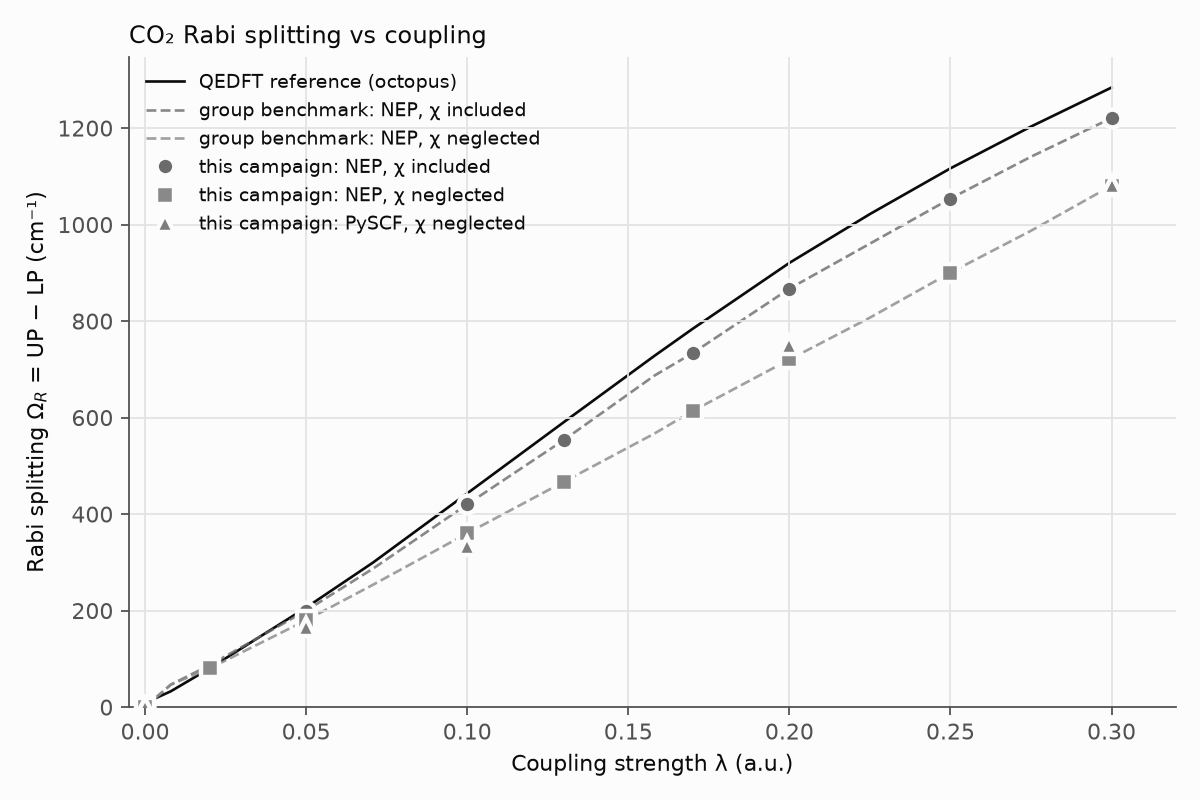
\includegraphics[width=\linewidth]{figures/co2_rabi_validation.png}
  \caption{Validation on a single CO$_2$ molecule: Rabi splitting versus coupling
  strength. Circles and squares, this work with NEP models with the polarizability
  included and neglected; triangles, PySCF with the polarizability neglected; dashed
  lines, benchmark of Ref.~\onlinecite{Li2026cboamd}; solid line, explicit CBOA QEDFT
  reference~\cite{Bonini2024}. \todo{redraw in final style; LDA vs.\ PBE0 for the
  PySCF points.}}
  \label{fig:co2}
\end{figure}

For a single water molecule with the cavity resonant with the bend, the bend splits
into two polaritons whose separation grows linearly with coupling,
$\Omega_R \approx 1265\,\lambda$~\cm\ with the polarizability neglected
(Fig.~\ref{fig:h2o}). With the polarizability included
($\chi_{xx}\approx 5.7$~a.u.), one polariton dominates and tracks the screened cavity
frequency $\omega/n_\text{eff}$, as for CO$_2$. Two features distinguish the polar
water molecule from CO$_2$. When the cavity polarization is tilted away from its
dipole, the molecule rotates appreciably, and a detuning scan lies 40--60~\cm\ below
the linear model that describes CO$_2$. \todo{resolve: origin of the offset (photon
initial condition, permanent dipole, anharmonicity); repeat for the O--H stretch;
resonant-protocol runs with $\chi$ included; longer runs.}

\begin{figure}[t]
  \centering
  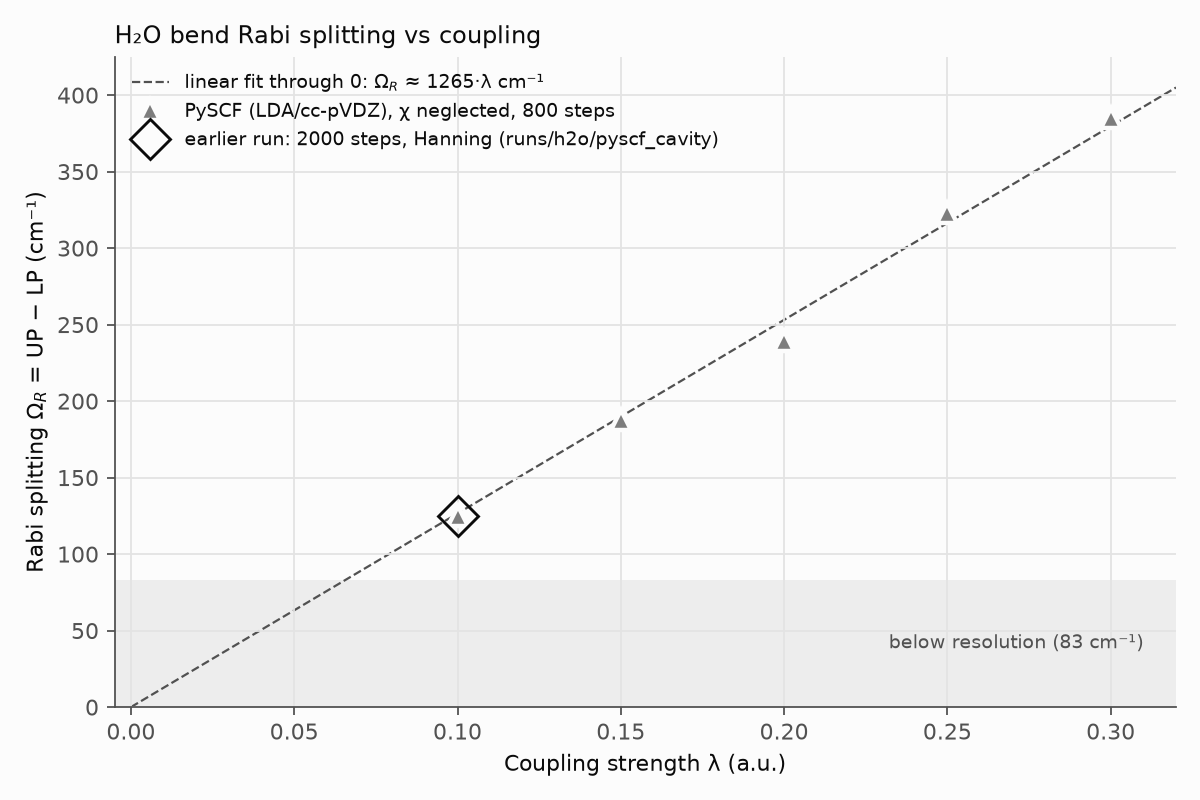
\includegraphics[width=\linewidth]{figures/h2o_rabi_single.png}
  \caption{Single water molecule (PySCF, LDA/cc-pVDZ, polarizability neglected) with the
  cavity resonant with the bend: Rabi splitting versus coupling strength, with a linear
  fit through the origin. The shaded band marks the frequency resolution of the
  800-step trajectories. \todo{replace with production level of theory and include the
  O--H stretch.}}
  \label{fig:h2o}
\end{figure}

\subsection{From one to a few molecules}
\label{sec:few}

\todo{Separation scan for $N=2$: bare spectra and splitting versus $R$; the distance
beyond which molecules couple only through the cavity. Collective scaling for $N=1$--4
at fixed $\lambda$ (expected $\Omega_R\propto\sqrt{N}$) and at $\lambda/\sqrt{N}$
(expected constant); role of orientation and rotation; dark modes.}

\begin{figure}[t]
  \centering
  \figplaceholder{4.2cm}{Rabi splitting versus $N$ (1--4) at fixed $\lambda$ and at
  $\lambda/\sqrt{N}$, with the $\sqrt{N}$ prediction; inset, splitting versus separation
  $R$ for $N=2$.}
  \caption{\todo{Collective scaling in small water clusters.}}
  \label{fig:few}
\end{figure}

\subsection{Liquid water: O--H stretch polaritons}
\label{sec:liquid}

\todo{IR spectra of liquid water versus coupling for the three protocols; Rabi
splitting versus $\lambda$ and its connection to the single-molecule value through
orientation and local-field factors; comparison with the experimental splitting;
upper-polariton linewidth versus coupling, compared with the narrowing reported in
Ref.~\onlinecite{Itatani2026}.}

\begin{figure}[t]
  \centering
  \figplaceholder{4.5cm}{IR spectra of liquid water in the O--H stretch region versus
  coupling: $\chi$ neglected, $\chi$ included at fixed $\omega$, and resonant protocol.}
  \caption{\todo{Polaritons of liquid water.}}
  \label{fig:liquid}
\end{figure}

\subsection{Hydrogen-bond network}
\label{sec:hbond}

\todo{Populations of network, intermediate and isolated water inside and outside the
cavity and their temperature dependence; whether the polarizable dynamics show the
retarded disordering seen experimentally while the $\chi$-neglected dynamics do not;
RDFs, hydrogen-bond lifetimes and correlation lengths; size of any effect relative to
statistical error.}

\begin{figure}[t]
  \centering
  \figplaceholder{4.5cm}{Fractions of network, intermediate and isolated water versus
  temperature, outside the cavity and inside it with $\chi$ neglected and included.}
  \caption{\todo{Hydrogen-bond populations under VSC.}}
  \label{fig:hbond}
\end{figure}

% ---------------------------------------------------------------------------
\section{Discussion}

\todo{Interpret the results against the experiment of Ref.~\onlinecite{Itatani2026}:
does the polarizability-mediated mechanism account for the observed network
reorganization, and at what coupling strength; what classical, mean-field CBOA dynamics
can and cannot capture (nuclear quantum effects, many cavity modes, cavity losses,
realistic molecule numbers); implications for cavity-modified chemistry in aqueous
solution.}

\section{Conclusions}

\todo{Three or four sentences: what we did, the main finding, and the outlook.}

\begin{acknowledgments}
\todo{Funding, computing resources (e.g.\ Flatiron Institute), and discussions.}
\end{acknowledgments}

\section*{Data availability}
Inputs, analysis scripts and data for all simulations are available at
\url{https://github.com/charliew0707/VSC_Molecular_Dynamics} \todo{archive with a DOI at
submission}; the simulation code is available at
\url{https://github.com/flickgroup/cboamd}.

% ---------------------------------------------------------------------------
\begin{thebibliography}{99}

\bibitem{Shalabney2015} A. Shalabney, J. George, J. Hutchison, G. Pupillo, C. Genet,
and T. W. Ebbesen, Coherent coupling of molecular resonators with a microcavity mode,
Nat. Commun. \textbf{6}, 5981 (2015).

\bibitem{Thomas2016} A. Thomas, J. George, A. Shalabney, M. Dryzhakov, S. J. Varma,
J. Moran, T. Chervy, X. Zhong, E. Devaux, C. Genet, J. A. Hutchison, and
T. W. Ebbesen, Ground-state chemical reactivity under vibrational coupling to the
vacuum electromagnetic field, Angew. Chem. Int. Ed. \textbf{55}, 11462 (2016).

\bibitem{Thomas2019} A. Thomas, L. Lethuillier-Karl, K. Nagarajan, R. M. A. Vergauwe,
J. George, T. Chervy, A. Shalabney, E. Devaux, C. Genet, J. Moran, and T. W. Ebbesen,
Tilting a ground-state reactivity landscape by vibrational strong coupling, Science
\textbf{363}, 615 (2019).

\bibitem{Xiang2020} B. Xiang, R. F. Ribeiro, M. Du, L. Chen, Z. Yang, J. Wang,
J. Yuen-Zhou, and W. Xiong, Intermolecular vibrational energy transfer enabled by
microcavity strong light--matter coupling, Science \textbf{368}, 665 (2020).

\bibitem{Ahn2023} W. Ahn, J. F. Triana, F. Recabal, F. Herrera, and B. S. Simpkins,
Modification of ground-state chemical reactivity via light--matter coherence in
infrared cavities, Science \textbf{380}, 1165 (2023).

\bibitem{Imperatore2021} M. V. Imperatore, J. B. Asbury, and N. C. Giebink,
Reproducibility of cavity-enhanced chemical reaction rates in the vibrational strong
coupling regime, J. Chem. Phys. \textbf{154}, 191103 (2021).

\bibitem{Wiesehan2021} G. D. Wiesehan and W. Xiong, Negligible rate enhancement from
reported cooperative vibrational strong coupling catalysis, J. Chem. Phys.
\textbf{155}, 241103 (2021).

\bibitem{Fukushima2022} T. Fukushima, S. Yoshimitsu, and K. Murakoshi, Inherent
promotion of ionic conductivity via collective vibrational strong coupling of water
with the vacuum electromagnetic field, J. Am. Chem. Soc. \textbf{144}, 12177 (2022).

\bibitem{Itatani2026} M. Itatani, N. Iwasa, K. Inaoka, N. Miyasaka, L. Takahashi,
K. Takahashi, T. Fukushima, M. Bamba, and K. Murakoshi, Hydrogen-bond network
reorganization in liquid water under vibrational strong coupling, arXiv:2606.12508
(2026). \todo{check reference once published}

\bibitem{Li2020PNAS} T. E. Li, J. E. Subotnik, and A. Nitzan, Cavity molecular dynamics
simulations of liquid water under vibrational ultrastrong coupling, Proc. Natl. Acad.
Sci. U.S.A. \textbf{117}, 18324 (2020).

\bibitem{Lieberherr2023} A. Z. Lieberherr, S. T. E. Furniss, J. E. Lawrence, and
D. E. Manolopoulos, Vibrational strong coupling in liquid water from cavity molecular
dynamics, J. Chem. Phys. \textbf{158}, 234106 (2023).

\bibitem{Bowles2025} J. Bowles, J. De La Fuente Diez, D. Laage, J. Richardi,
R. Vuilleumier, and R. Spezia, Liquid water under vibrational strong coupling: An
extended cavity Born--Oppenheimer molecular dynamics study, J. Chem. Phys.
\textbf{163}, 044104 (2025).

\bibitem{Li2020JCP} T. E. Li, A. Nitzan, and J. E. Subotnik, On the origin of
ground-state vacuum-field catalysis: Equilibrium consideration, J. Chem. Phys.
\textbf{152}, 234107 (2020).

\bibitem{Flick2017} J. Flick, H. Appel, M. Ruggenthaler, and A. Rubio, Cavity
Born--Oppenheimer approximation for correlated electron--nuclear-photon systems,
J. Chem. Theory Comput. \textbf{13}, 1616 (2017).

\bibitem{Bonini2024} J. Bonini, I. Ahmadabadi, and J. Flick, Cavity Born--Oppenheimer
approximation for molecules and materials via electric field response, J. Chem. Phys.
\textbf{161}, 154104 (2024).

\bibitem{Li2026cboamd} Y. Li, R. Car, and J. Flick, cboamd: A machine learning molecular
dynamics framework for vibrational strong coupling, arXiv:2609.22022 (2026).

\bibitem{ASE2017} A. Hjorth Larsen \textit{et al.}, The atomic simulation
environment---a Python library for working with atoms, J. Phys.: Condens. Matter
\textbf{29}, 273002 (2017).

\bibitem{PySCF2018} Q. Sun \textit{et al.}, PySCF: the Python-based simulations of
chemistry framework, WIREs Comput. Mol. Sci. \textbf{8}, e1340 (2018).

\bibitem{Zhang2020} L. Zhang, M. Chen, X. Wu, H. Wang, W. E, and R. Car, Deep neural
network for the dielectric response of insulators, Phys. Rev. B \textbf{102}, 041121
(2020).

\bibitem{Sommers2020} G. M. Sommers, M. F. C. Andrade, L. Zhang, H. Wang, and R. Car,
Raman spectrum and polarizability of liquid water from deep neural networks, Phys.
Chem. Chem. Phys. \textbf{22}, 10592 (2020).

\bibitem{DeePMD2023} J. Zeng \textit{et al.}, DeePMD-kit v2: A software package for deep
potential models, J. Chem. Phys. \textbf{159}, 054801 (2023).

\end{thebibliography}

\end{document}
